\chapter{Hardware}
\label{chap_hardware}

SCAS hardware provides programmable communication paths between different interfaces while maximising the throughput.
From an abstract point of view, SCAS can be seen as a form of crossbar switch (although not entirely true) interfaced with standard PCIe, DRAM, and Ethernet interfaces and a scalable AXI4-Stream based user logic interface.
The PCIe interface supports up to x4 PCIe Gen.2 standard, the DRAM interface supports up to 1GB DDR3-800 SODIMM modules and the Ethernet interface supports 1Gbit (Gigabit) raw Ethernet communication bandwidth.

\begin{figure}[h]
\centering
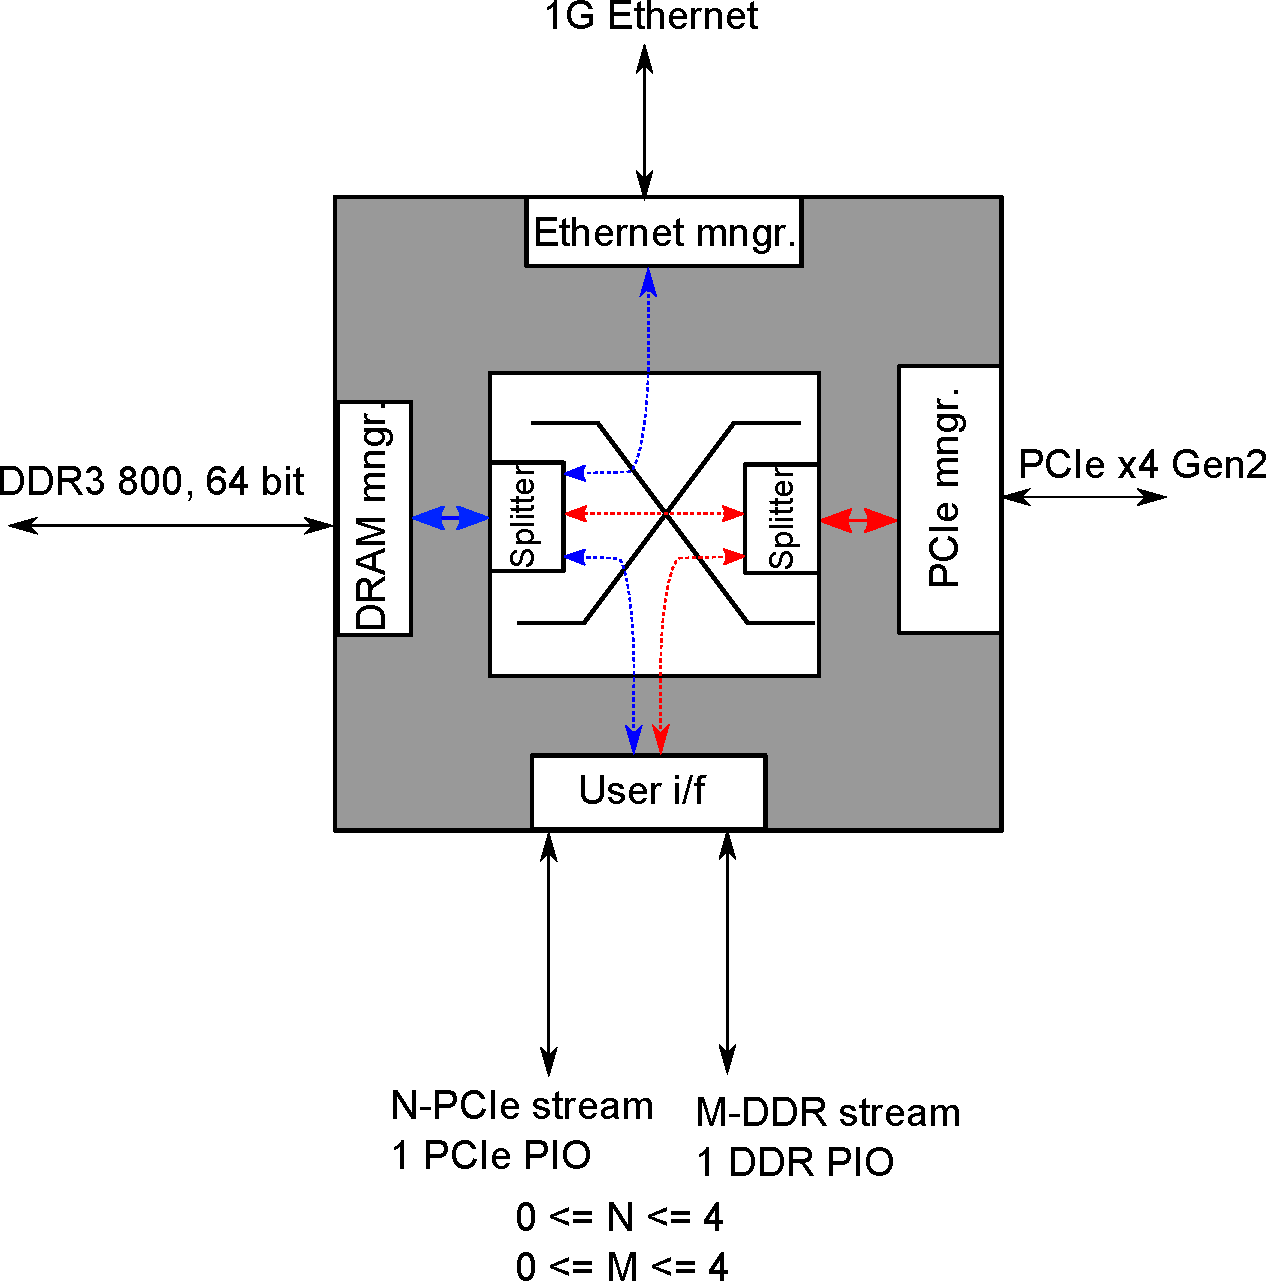
\includegraphics[width=8cm]{figures/switch.pdf}
\caption{Switch Architecture.}
\label{fig:switch_arch}
\end{figure}

\noindent The user interface supports 64-bit wide AXI4-Stream interfaces from both PCIe and DRAM (User PCIe Stream interface and User DRAM Stream interface).
The number of AXI4-Stream channels can be configured between 0 and 4 for both PCIe and DRAM.
The interface clock frequency to user logic for these stream interfaces are run-time reconfigurable and it defaults to 250MHz.
An abstract view of the switch architecture is given in Fig.~\ref{fig:switch_arch}.

The valid communication pathways for SCAS are shown in table~\ref{tab:cm_paths}.
The host system where the SCAS FPGA card is plugged in can directly communicate to the on-board DRAM and the user interface.
Presently communication through Ethernet is supported only from/to the DRAM.
Concurrent communication operations are possible and are managed within the FPGA logic and the driver software.
Generally user application does not have to bother about communication pathways interacting and causing data corruption or bottlenecks.
Some of the possible contention scenarios are described in Chapter~\ref{chap_integration}.
Detailed description of hardware modules are provided in the following sections.
For developing applications or using SCAS, users do not have to understand these low level details.
These are provided to encourage developers who would like to customise SCAS for their specific use cases.

\input \TBLDIR/communication_paths.tex

\section{PCIe manager}
The PCIe manager module manages all the data communication between the host system and the FPGA through PCIe interface.
The major sub-modules within this block are shown in Fig.~\ref{pcie_mnger}.
\begin{figure}[h]
\centering
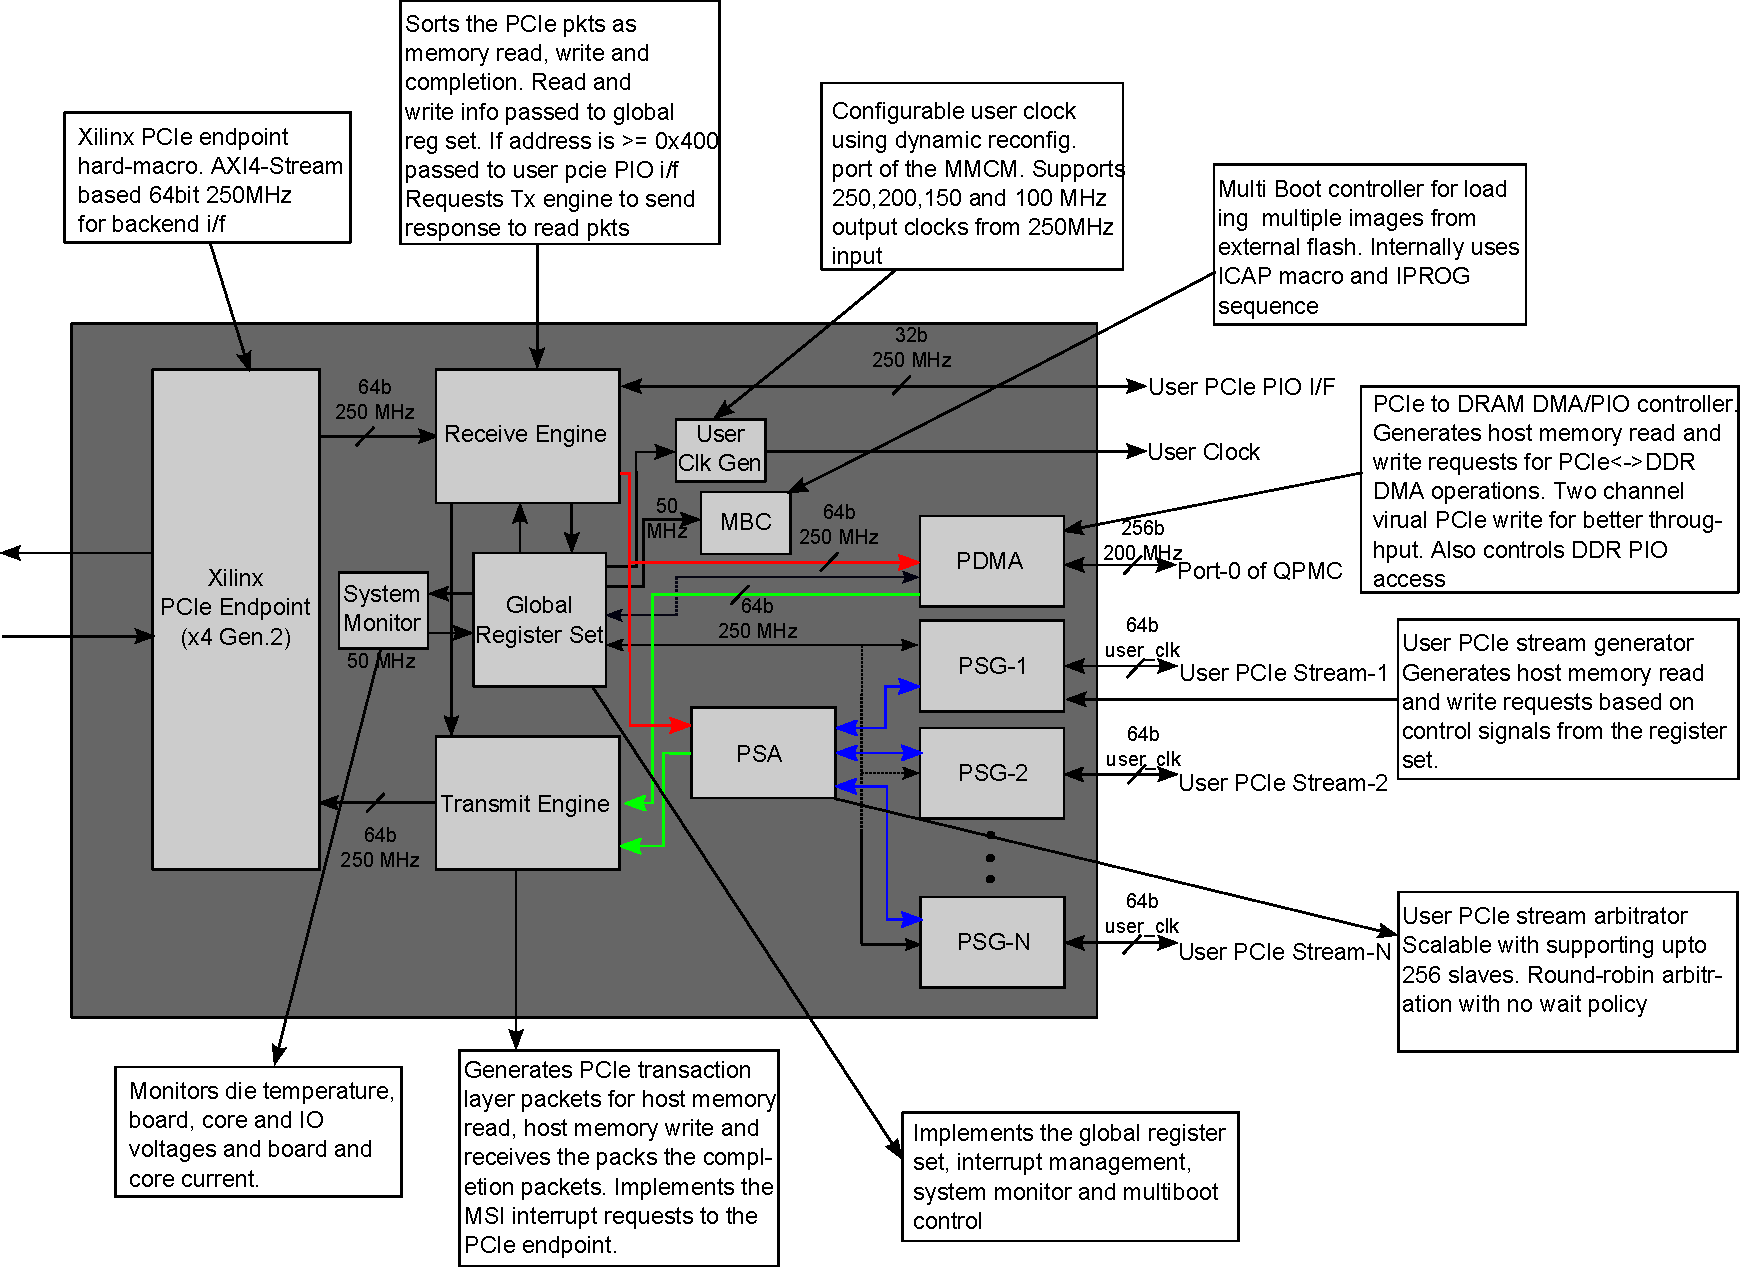
\includegraphics[width=16cm]{figures/pcie_section.pdf}
\caption{PCIe Manager Architecture.}
\label{pcie_mnger}
\end{figure}

\subsection{PCIe Endpoint block}
This module uses the Xilinx PCIe Endpoint hard block configured in PCIe Gen.2 configuration with x4 link width.
This is the highest configuration supported in the Virtex-6 FPGAs although Virtex-7 devices supports PCIe Gen.2 in x8 configuration.
Theoretically PCIe x4 Gen.2 configuration can give a maximum throughput of 2GBytes/sec per direction in full-duplex mode.
The present configuration settings enable high-portability of user applications irrespective of the target FPGA.
The endpoint block implements the lower layers of PCIe protocol such as the data link layer and the physical layer.
The physical layer uses Xilinx's GTP tranceivers.
The maximum payload size for the PCIe core is set to 256bytes and the core uses 4 internal BRAM based buffers to store the PCIe packets.
The backend of the Endpoint is integrated with the fabric using AXI4-Stream interface to generate and consume PCIe packets from the upper layers.

\subsection{PCIe transaction layer}
The Endpoint block is directly interfaced with the receive and transmit engines, which act as the transaction layer for the PCIe protocol.
Transaction layer generates and consumes packets called transaction layer packets (TLPs), which are the unit of communication in PCIe.
The interface to the transaction layer is 64bits wide and runs at 250MHz clock frequency provided by the Endpoint.
The receive engine (Rx engine) decodes the received TLPs and route them to the appropriate sub modules.
The received TLPs may correspond to a memory read requests, memory write requests or a completion packets resulting from a memory read request issued by the FPGA.
If the memory write request is for an address location less than 0x400, it is routed to the global register set else it is directed to the user PCIe PIO interface.
Similarly for memory read requests, the request is forwarded to the global register or the user PCIe PIO interface depending upon the address and also triggers the transmit engine (Tx engine) to send the completion packet corresponding to this request with the data from the requested location.

From the completion packets, Rx engine extracts and packs the data and streams it out along with the \emph{tag number} in the received packet.
Tag number is a field in the PCIe packet inserted by a read operation initiator.
The device which responds to a read request should keep this same tag number in the completion packet, which enables the initiator to determine the specific request which generated this packet.
This is particularly useful when there are multiple outbound read requests.

The Tx engine generates TLPs corresponding to memory read, memory write and completion.
Memory read TLPs are generated during DMA operations to fetch data from host memory to the FPGA.
Memory write TLPs are generated while transmitting data from FPGA to the host memory and completion TLPs are generated in response to PIO read requests from the host.
The Tx engine also manages PCIe interrupts to the host (known as message signaled interrupt (MSI)) based on the request from the interrupt manager in the global register set.

\subsection{Global Register Set}
Table~\ref{tab:reg_set} lists the global register space of SCAS.
The PCIe endpoint device is configured to request for 4MBytes in the host system memory address space.
The first 0x3FC is reserved for the global register space and any access from the host above 0x3FC is routed to the user PCIe PIO interface.
If more memory space is required by the user application, the Xilinx PCIe endpoint IP has to be regenerated.
The details of regenerating the IP cores are described in Chapter~\ref{chap_customisation}.
Users are also free to add additional registers in the global set if required.

\input \TBLDIR/reg_set.tex

This module also implements the interrupt manager.
The interrupt manager makes sure that multiple back to back interrupts are not sent to the host in case of concurrent data transfer operations since this may sometimes crash the host or cause interrupt misses.
The manager queues the interrupt requests and clears the interrupts which are acknowledged by the host.
The host acknowledges interrupts by write clearing the status register (0x10) when it detects an interrupt.
\subsection{System Monitor}
System monitor is used to monitor the system health parameters such as temperature and power consumption.
It uses the Xilinx's System monitor hard macro along with on-board sensors.
These parameters can be accessed from the host system using an API (\emph{fpga\_read\_sys\_param()}).
The readings obtained from the System monitor are converted to actual values by the driver software using Xilinx specific transfer functions.
This monitoring functionality is available only on ML605 board since there are no on-board sensors on VC707 board.

\subsection{User Clock Generator}
This module generates the clock frequency used for all user stream interfaces.
There may be situations where the user logic cannot work at the system clock frequency.
This module takes the 250MHz clock from the PCIe core as the input and generates the output frequency depending upon an API request (\emph{user\_set\_clk()}).
Presently the supported output frequencies are 250,200,150 and 100MHz.
Internally this module uses the dynamic reconfiguration port (DRP) of an mixed-mode clock manager (MMCM) to derive the required clock frequency.
Using dedicated MMCM for user clock generation makes sure that other clock signals are not disrupted during clock reconfiguration.

\subsection{Multiboot Controller}
The multiboot controller (MBC) helps to reconfigure the FPGA by loading a new bitstream from the external storage memory (Platform Flash or BPI).
Internally the MBC instantiates Xilinx's ICAP primitive and uses the \emph{IPROG} command sequence to trigger a reconfiguration operation.
The application software uses the \emph{fpga\_reboot()} API to trigger a reconfiguration operation by specifying the starting address of bitstream in the memory.
The ML605 board is equipped with both Platform Flash as well as the BPI flash and VC707 board has only a BPI flash.
On VC707, while storing the bitstream in the BPI flash, it should be noted that the starting address-bitstream size combination should not cross 32MBytes since the BPI is partitioned into four region using the FPGA version selection pins.

\subsection{PCIe-DRAM DMA/PIO controller (PDMA)}
This module is responsible controlling data movement between the PCIe controller and the external DRAM memory.
This can access DRAM in both PIO (address/data) and DMA modes.
This module is configured by the registers in the global register space.
This module implements two virtual channels for host-DRAM write operations to achieve better performance.
In some applications PCIe write (host to FPGA) performance is lower due to some restrictions of the PCIe protocol.
As per PCIe standard, the maximum data that can be requested by an endpoint from the host in a single request is 4KB (or maximum read request size set by the host in the PCIe endpoint configuration space).
For large data transfers, this makes the endpoint to make several requests.
When an endpoint point makes multiple outstanding requests, the protocol provides the host the flexibility to return the completion packets in any order, irrespective of the requested order.
This is called out-of-order completion.
If the endpoint cannot manage this scenario, it is forced to make a new request only after receiving the data for the previous request.
This can severely affect system performance.
To overcome this issue, SCAS make use of the \emph{tag} number in PCIe packet.
Each time a memory request is made to the host, the request is tagged with a specific number.
As per the protocol, the completion packet returned for each request should maintain the tag number unaltered.
This enables reassembling data in correct order by PDMA.
Experiments showed that implementing only two such virtual channels will provide sufficiently high throughput performance.
Asymmetric FIFOs are used to convert 64bit wide PCIe interface data stream to 256bit wide DRAM interface data stream.

\subsection{PCIe Stream Generator (PSG)}
This module generates AXI-streams to the user PCIe-stream interface.
It is responsible for making data requests to the host system for transferring data from host to user stream interfaces and vice versa.
PSG instantiates asynchronous FIFOs between the user interface and PCIe data managers, which enables running the user PCIe stream interface at a different clock frequency than the PCIe core frequency.
The number of PSGs instantiated in SCAS depends upon the number of user PCIe stream interfaces specified by the user.
The FIFOs within PSGs are 8KB in size and a PSG never initiates a PCIe read or write operation unless there is sufficient buffer to store data.
This avoids creating deadlocks in the PCIe core.
For example if PSG requests for data without checking the space in the local FIFO and the user application stops receiving data from PSG, the PCIe core is stalled until the user application starts accepting data.

\subsection{PSG Stream Arbitrators (PSA)}
This module arbitrates among different PSGs.
It employs round-robin-arbitration among the streams to access the PCIe core controller.
It is highly scalable with current implementation supporting up to 256 PSGs.

\section{DRAM manager}
DRAM manger controls communication between the PCIe manager, user DRAM interface and the Ethernet manager with the external DRAM memory.
\subsection{DDR Controller}
This module instantiates the Xilinx's DDR3 soft memory controller.
It is generated using Xilinx's memory interface generator (MIG) available with the IP Core generator.
The controller is configured to control a 1GB DDRM SODIMM module running at 400MHz I/O clock frequency.
Its backend is a custom interface defined by Xilinx which is 256bits wide and runs at 200MHz.
\subsection{Four port memory controller (FPMC)}
This is the most important component of DRAM manager.
This module multiplexes DRAM access from different sources.
It has four identical ports which are interfaced to PCIe-DRAM DMA/PIO controller (PDMA), User DRAM PIO interface, User DRAM stream arbitrator (DSA) and the Ethernet manager.
Requests from these sources are served in round-robin-arbitration scheme.
Since the DDR controller has a single request port for access request, read-write request from each port is also served based on round robin.
For better system performance, FPMC allows back-to-back DRAM read requests and internally stores them in a tracking buffer.
When data is received from the DDR controller, it is routed to the appropriate port based on this tracking information.
\subsection{DRAM Stream Generator (DSG)}
DRAM stream generators control the DRAM-User logic AXI stream interfaces.
They are quite similar to PSGs except the fact that their user side interface is 64bits wide and DRAM interface side is 256bits wide.
Currently Xilinx does not support asymmetric (different read and write width) AXI Fifos.
Hence DSGs use two FIFOs with intermediate logic to convert interface widths.
The number of DSGs instantiated in the design depends upon the number of User DRAM stream interfaces specified by the user.
The FIFOs also enable the user DRAM stream interface to work at a different frequency than the DRAM core frequency.

\subsection{DSG stream arbitrator (DSA)}
DSG arbitrates requests from DSGs in a round-robin fashion.
DSG also implements a tracking buffer similar to the FPMC, which enables accepting back-to-back read requests from different DSGs.
\begin{figure}[t]
\centering
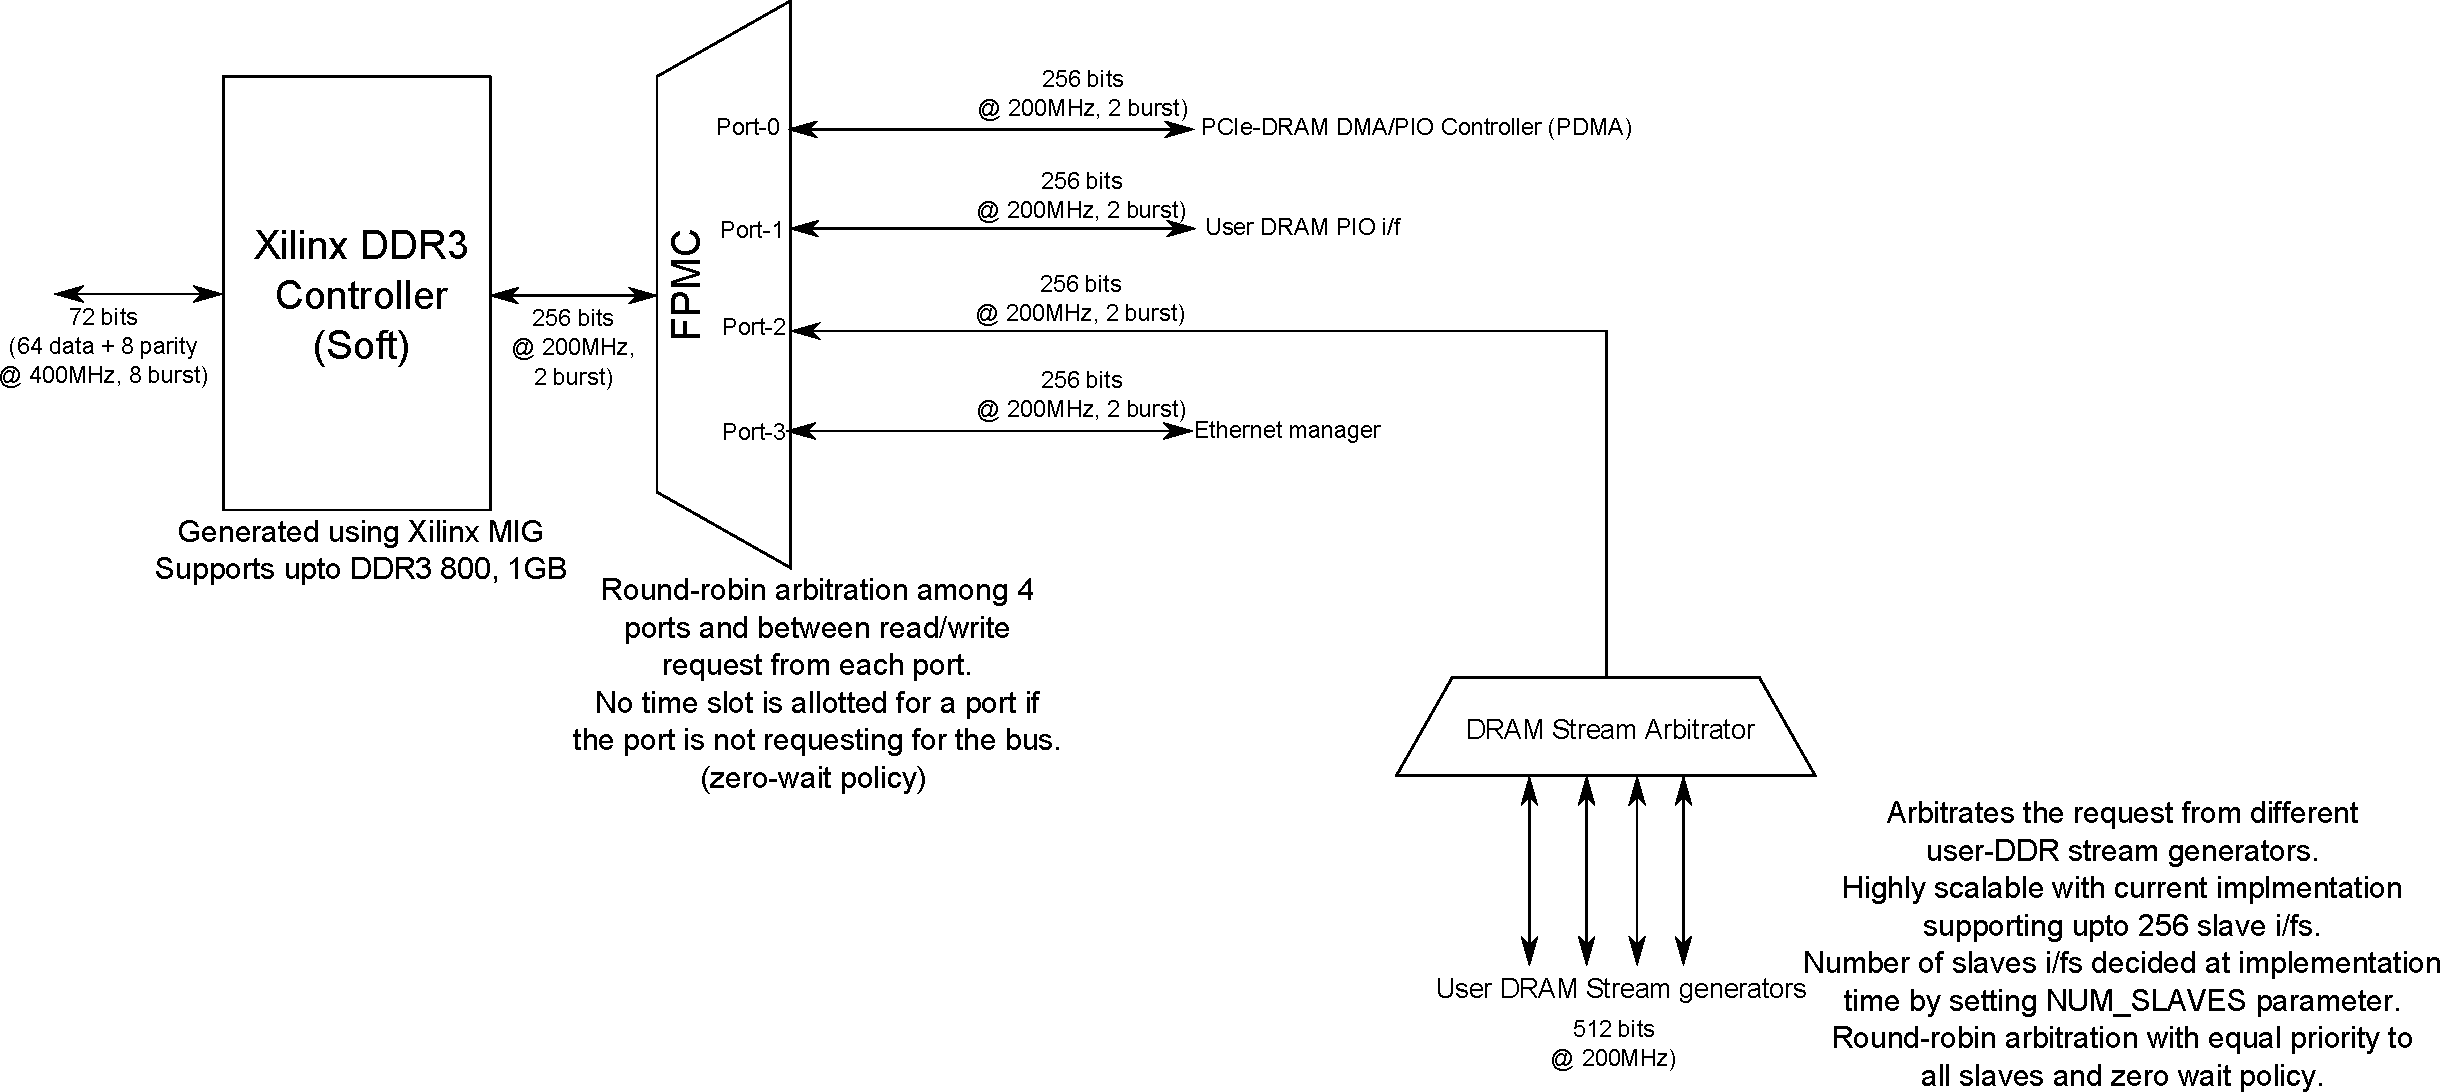
\includegraphics[width=16cm]{figures/ddr_arbitration.pdf}
\caption{DRAM Manager Architecture.}
\label{exe_model}
\end{figure}

\section{Ethernet manager}
The Ethernet manager control data movement between the DRAM manager and the Ethernet interface.
For Virtex-6, the Ethernet control used is a hard Tri-mode Ethernet MAC, where as Virtex-7 uses a soft Ethernet core.
The Virtex-7 Ethernet core requires special license from Xilinx for core as well as bitstream generation.
Ethernet manager has sub modules which perform Ethernet specified packing and unpacking of data and FIFOs and associated control logic to manage interface width mismatch.


\section{User Interface}
The user interface includes PCIe stream interfaces, DRAM stream interfaces, PCIe PIO interface, DRAM PIO interface and the interrupt interface.
The user interface signals are described in Table~\ref{tab:user_sigs}.

\input \TBLDIR/user_if_signals.tex

All the streaming interfaces (PCIe and DRAM) interface works at \emph{i\_user\_clk} frequency domain, whose default value is 250MHz.
The PCIe PIO interface as well as the interrupt interface works at the PCIe core frequency (250MHz).
The DRAM PIO interface works at DRAM core frequency, which is 200MHz.







